\documentclass[12pt]{article}
\usepackage[margin=2.5cm]{geometry}
\usepackage{enumerate}
\usepackage{amsfonts}
\usepackage{amsmath}
\usepackage{fancyhdr}
\usepackage{amsmath}
\usepackage{amssymb}
\usepackage{amsthm}
\usepackage{mdframed}
\usepackage{graphicx}
\usepackage{subcaption}
\usepackage{adjustbox}
\usepackage{listings}
\usepackage{xcolor}
\usepackage{booktabs}
\usepackage[utf]{kotex}

\definecolor{codegreen}{rgb}{0,0.6,0}
\definecolor{codegray}{rgb}{0.5,0.5,0.5}
\definecolor{codepurple}{rgb}{0.58,0,0.82}
\definecolor{backcolour}{rgb}{0.95,0.95,0.92}

\lstdefinestyle{mystyle}{
    backgroundcolor=\color{backcolour},
    commentstyle=\color{codegreen},
    keywordstyle=\color{magenta},
    numberstyle=\tiny\color{codegray},
    stringstyle=\color{codepurple},
    basicstyle=\ttfamily\footnotesize,
    breakatwhitespace=false,
    breaklines=true,
    captionpos=b,
    keepspaces=true,
    numbers=left,
    numbersep=5pt,
    showspaces=false,
    showstringspaces=false,
    showtabs=false,
    tabsize=1
}

\lstset{style=mystyle}

\begin{document}
\title{CSC148 Midterm Version 1 Solution}
\author{Hyungmo Gu}
\maketitle

\section*{Question 1}
\begin{enumerate}[a.]
    \item

    \adjustbox{center, valign=t}{
    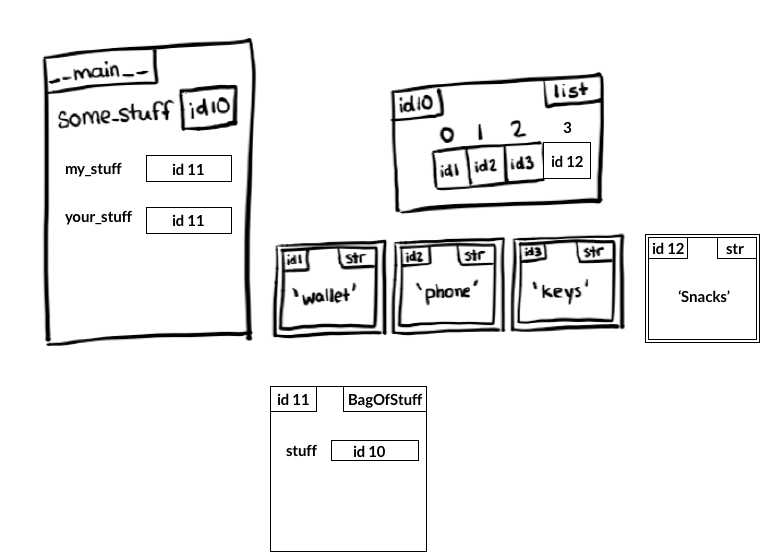
\includegraphics[width=0.8 \linewidth]{images/midterm_version_1_q1a_solution.png}
    }

    \newpage

    \begin{mdframed}
        \underline{\textbf{Correct Solution:}}

        \bigskip

        \adjustbox{center, valign=t}{
        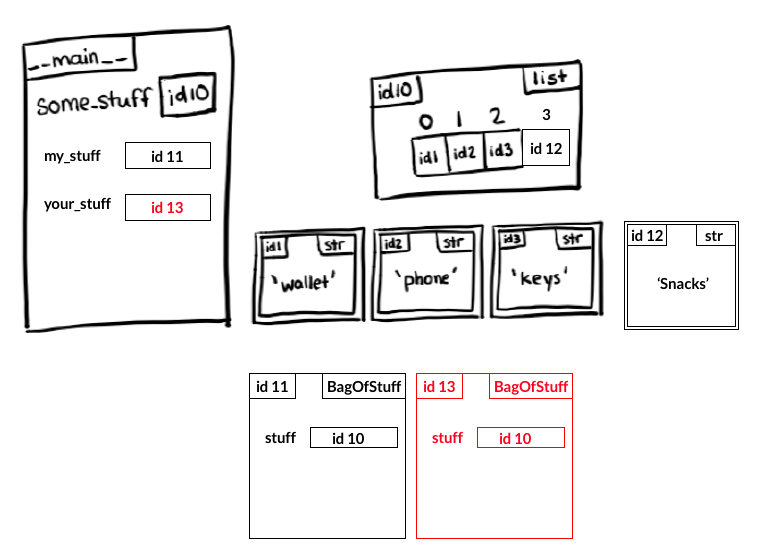
\includegraphics[width=0.8 \linewidth]{images/midterm_version_1_q1a_correction.png}
        }
    \end{mdframed}

    \item

    First, we need to write what causes the assertion to fail

    \bigskip

    The assertion fails because the instance attribute \textit{stuff} in two
    different instances of class `BagOfStuff' are pointing to the same list.

    \bigskip

    Second, we need to write down how to fix this issue.

    \bigskip

    To fix this issue, we need make sure \textit{stuff} don't point to the list in
    same memory location. This is done by changing the line from

    \bigskip

    \begin{lstlisting}[language=python]
    self.stuff = stuff
    \end{lstlisting}

    to

    \begin{lstlisting}[language=python]
    self.stuff = [x for x in stuff]
    \end{lstlisting}



\end{enumerate}

\section*{Question 2}
\begin{itemize}
    \item
    \adjustbox{center, valign=t}{
        \begin{tabular}{|c|c|c|c|c|}
            \hline
            Class 1 & Class 2 & Composition? & Inheritance? & Neither?\\
            \hline
            Chirper & Cheep & & x & \\
            \hline
            Customer & Item & x & & \\
            \hline
            ExpressLine & Customer & x & & \\
            \hline
            ExpressLine & SelfServeLine & & x & \\
            \hline
            PriorityQueue & Container & & & x \\
            \hline
            GroceryStore & GroceryStoreSimulation & x & & \\
            \hline
        \end{tabular}
    }

    \bigskip

    \begin{mdframed}
        \underline{\textbf{Correct Solution:}}

        \bigskip

        \begin{tabular}{|c|c|c|c|c|}
            \hline
            Class 1 & Class 2 & Composition? & Inheritance? & Neither?\\
            \hline
            Chirper & Cheep & \color{red}x\color{black} & & \\
            \hline
            Customer & Item & x & & \\
            \hline
            ExpressLine & Customer & x & & \\
            \hline
            ExpressLine & SelfServeLine & & & \color{red}x\color{black} \\
            \hline
            PriorityQueue & Container & & \color{red}x\color{black} & \\
            \hline
            GroceryStore & GroceryStoreSimulation & x & & \\
            \hline
        \end{tabular}
    \end{mdframed}

    \bigskip

    \underline{\textbf{Notes:}}

    \begin{itemize}
        \item Learned that composition is commonly thought as `has a' relationship
        \item Learned that inheritance is commonly thought as `is a' relationship
    \end{itemize}

    \item


\end{itemize}

\section*{Question 3}

\section*{Question 4}

\section*{Question 5}

\section*{Question 6}

\section*{Question 7}

\end{document}